\setcounter{figure}{0}
\renewcommand{\thefigure}{A\arabic{figure}}

\begin{figure}[htpb!]
\begin{center}
\caption{Proportion of Twins by Birth Order}
\label{TWINfig:bord}
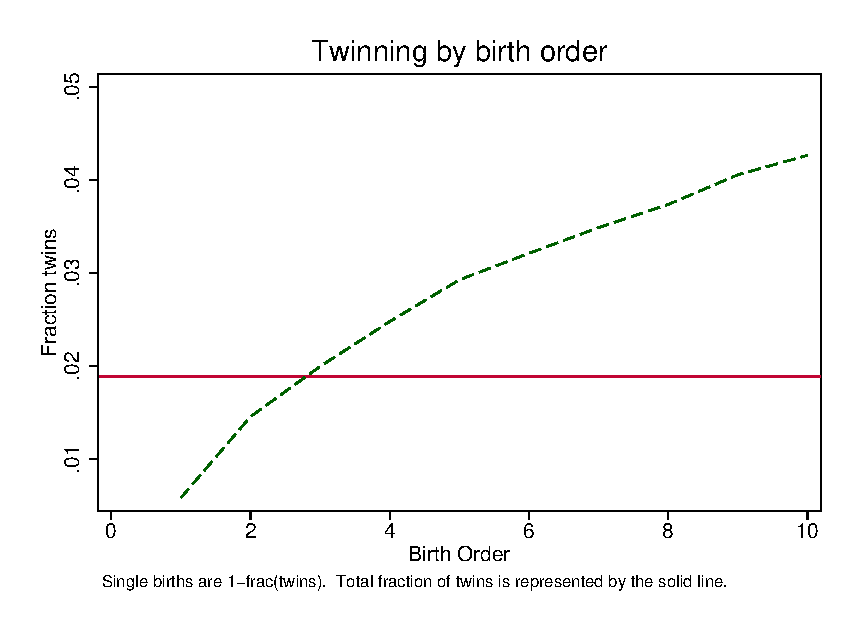
\includegraphics[scale=0.92]{\twinfolder/Figures/twinbybord.eps} 
\end{center}
\end{figure}

\begin{figure}[htpb!]
\begin{center}
\caption{Birth Size of Twins versus Singeltons}
\label{TWINfig:Size}
\includegraphics[scale=0.90]{\twinfolder/Figures/Size.eps} 
\end{center}
\end{figure}

\begin{figure}[htpb!]
\begin{center}
\caption{Height and Selective Survival}
\label{TWINfig:survival}
\includegraphics[scale=0.90]{\twinfolder/Figures/MMRcuts.eps} 
\end{center}
\end{figure}

\begin{figure}[htpb!]
\begin{center}
\caption{Relaxing the Exclusion Restriction (four plus)}
\label{TWINfig:ltz4}
\includegraphics[scale=0.90]{\twinfolder/Figures/LTZ_four.eps} 
\end{center}
\floatfoot{Note to figure \ref{TWINfig:ltz4}: See notes to figure
\ref{TWINfig:ltz3}}
\end{figure}

\begin{subfigures}
\begin{center}
\begin{figure}
\caption{Bootstrap Estimates of $\hat\gamma$ (Normal)}
\label{TWINfig:gammaBootsN}
\includegraphics[scale=0.90]{\twinfolder/Figures/gammaResamp.eps} 
\end{figure}

\begin{figure}
\caption{Bootstrap Estimates of $\hat\gamma$ (log Normal)}
\label{TWINfig:gammaBootsL}
\includegraphics[scale=0.90]{\twinfolder/Figures/gammaLogN.eps} 
\floatfoot{Note to figures \ref{TWINfig:gammaBootsL}-\ref{TWINfig:gammaBootsN}: 
The empirical distributionis generated by performing J=100 bootstrap replications 
to estimate $\phi^t$ and $\phi^q$ (see discussion in appendix \ref{TWINscn:gamma}).  
The overlaid analytical distribution in figure A is normal $\sim N(\mu_{\hat\gamma},
\sigma_{\hat\gamma})$, and in figure B is log Normal with the same mean and 
standard deviation.  The first and second moments estimated in the bootstrap 
replications are $\mu_{\hat\gamma}=0.00898$ and $\sigma_{\hat\gamma}=0.00265$.}
\end{figure}
\end{center}
\end{subfigures}
